\subsection{Data Preprocessing}
The constructed \textbf{DRE19} dataset consists of images of varying resolutions; all images are full color. 
In order for the images to be passed into pretrained models, all images were rescaled to a (224, 224, 3) resolution - which appears to be the standard format.
\\
In determining the most model-performant image augmentations, all models were trained and evaluated with both a simple preprocessing procedure and a more advanced image preprocessing procedure. 

\paragraph{Simple Image Augmentation} ~\\
The default image augmentation scheme involves two image preprocessing steps; rescaling the image to conform with the (224, 244, 3) format and normalizing pixel values by dividing the image array by 255. 
The pixel normalization ensures that all values in the image array are constrained to the range $[0,1]$. 
Pixel normalization is a common transformation which achieves lower combinatorial span and thus reduces memory required for model training.

\paragraph{ImageNet Image Augmentation Configuration}\label{par:resnet50} ~\\
The ResNet50 image augmentation scheme operates slightly differently depending on the input type and \texttt{keras.backend} configuration - this will not be discussed further. 
Utilizing \texttt{keras.applications.resnet50.preprocess\_input} subtracts the mean RGB-channel values of the entire \texttt{imagenet} dataset from the provided input. 
The RGB-channel means for ImageNet are $[103.939, 116.779, 123.68]$\footnote{\href{https://github.com/keras-team/keras-applications/tree/8a1e4d427999c26d1a1988dda45454769c4372a5/keras_applications}{keras.applications source code}}.

\paragraph{Places Image Augmentation Configuration} ~\\
VGG16 pretrained on \texttt{places365}\autocite{gkallia2017keras_places365} uses a similar strategy to the \nameref{par:resnet50}, but centers the RBG values around the mean RGB-channel values for the Places dataset. 
RGB-channel means for Places $[104.006, 116.669, 122.679]$ \footnote{\href{https://github.com/GKalliatakis/Keras-VGG16-places365/commit/bdadf6a4ddbb1cc56e6826f0bb375bafd3cd0c1a#diff-a6d65babe02b4e2cca2d2c981f7e1e7f}{github.com/GKalliatakis/Keras-VGG16-places365}}- which imply that colors in the red and blue spectrum are slightly more prevalent in the Places dataset compared to ImageNet.

\subsubsection{Comparing augmentation schemes}
From \autoref{fig:preprocessing_images}, it is clear, that the choice of image augmentation scheme has significant repercussions for what features a model is inclined to learn. 

\begin{figure}[H]
    \centering
    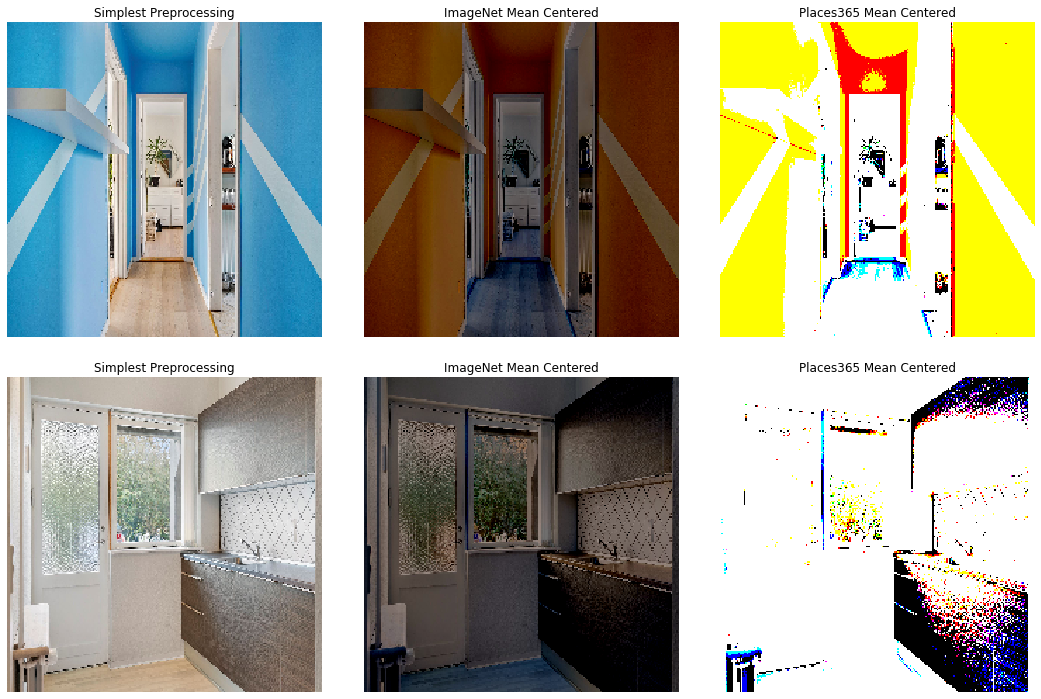
\includegraphics[scale=0.3]{pictures/plots/image2_preprocessing}
    \caption{The 3 Preprocessing Schemes}
    \label{fig:preprocessing_images}
\end{figure}

It appears, that the Places image augmentation picks up lighting in rooms in a more pronounced way in both sample images - this could be a contributing factor for detecting commonalities in human-perceived aesthetics. 